\section{Planos Tangentes}

En el cálculo de una variable, la recta tangente a $y = f(x)$ en $x_0$ es la mejor aproximación lineal de la función en ese punto. En dos variables, el análogo es el plano tangente a la superficie $z = f(x, y)$ en un punto dado: el plano que mejor aproxima a la superficie en un entorno de ese punto.

\subsection{Derivación de la ecuación}

Un plano que pasa por el punto $(x_0, y_0, z_0)$ con $z_0 = f(x_0, y_0)$ tiene la forma:
\[
z - z_0 = a(x - x_0) + b(y - y_0)
\]
para ciertos coeficientes $a$ y $b$ por determinar. El criterio de tangencia exige que este plano contenga las rectas tangentes a las curvas de corte de la superficie con cada plano coordenado vertical.

La intersección del plano con $y = y_0$ produce la recta $z - z_0 = a(x - x_0)$. Esa recta debe ser tangente a la curva $z = f(x, y_0)$ en $x_0$, por lo que su pendiente es $f_x(x_0, y_0)$, de donde $a = f_x(x_0, y_0)$.

La intersección con $x = x_0$ produce la recta $z - z_0 = b(y - y_0)$. Por el mismo argumento, $b = f_y(x_0, y_0)$.

Sustituyendo ambos coeficientes se obtiene la ecuación del plano tangente.

\begin{mydefinition}{Plano tangente}
Sea $f: D \subseteq \mathbb{R}^2 \to \mathbb{R}$ diferenciable en $(x_0, y_0)$. El plano tangente a la superficie $z = f(x, y)$ en el punto $(x_0, y_0, f(x_0, y_0))$ es:
\[
z = f(x_0, y_0) + f_x(x_0, y_0)\,(x - x_0) + f_y(x_0, y_0)\,(y - y_0)
\]
\end{mydefinition}

\begin{center}
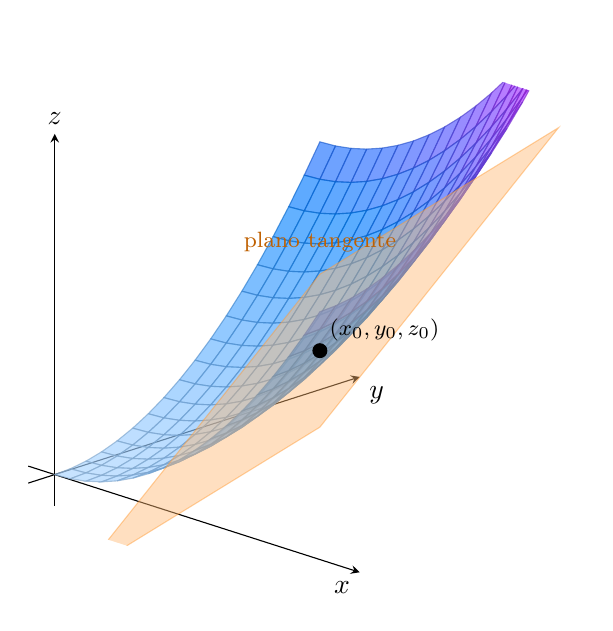
\begin{tikzpicture}
\begin{axis}[
    view={45}{22},
    axis lines=center,
    xlabel={$x$}, ylabel={$y$}, zlabel={$z$},
    xlabel style={anchor=north east},
    ylabel style={anchor=north west},
    zlabel style={anchor=south},
    xmin=-0.2, xmax=2.3,
    ymin=-0.2, ymax=2.3,
    zmin=-0.5, zmax=5.5,
    xtick=\empty, ytick=\empty, ztick=\empty,
    width=10cm, height=9cm,
]
    % Paraboloide z = x^2 + y^2
    \addplot3[
        surf, opacity=0.65,
        domain=0:2, domain y=0:2,
        samples=18,
        colormap/cool,
    ] {x^2 + y^2};

    % Plano tangente z = 2x + 2y - 2 en (1,1,2)
    \addplot3[
        surf, opacity=0.45,
        domain=0.1:1.9, domain y=0.1:1.9,
        samples=2,
        shader=flat,
        fill=orange!55,
        draw=orange!80,
    ] {2*x + 2*y - 2};

    % Punto de tangencia
    \addplot3[mark=*, mark size=2.5pt, black] coordinates {(1,1,2)};

    \node[font=\footnotesize, orange!75!black] at (axis cs:0.3, 1.7, 2.8)
        {plano tangente};
    \node[font=\footnotesize, black, anchor=south west] at (axis cs:1,1,2)
        {$(x_0, y_0, z_0)$};
\end{axis}
\end{tikzpicture}
\end{center}

\subsection{Aproximación lineal}

La ecuación del plano tangente proporciona una forma de aproximar $f(x, y)$ cuando $(x, y)$ es cercano a $(x_0, y_0)$. Dado que el plano se acerca a la superficie en ese entorno, se tiene:
\[
f(x, y) \approx f(x_0, y_0) + f_x(x_0, y_0)(x - x_0) + f_y(x_0, y_0)(y - y_0)
\]

La función del lado derecho se denomina linealización de $f$ en $(x_0, y_0)$.

\begin{mydefinition}{Linealización}
La linealización de $f$ en $(x_0, y_0)$ es la función afín:
\[
L(x, y) = f(x_0, y_0) + f_x(x_0, y_0)(x - x_0) + f_y(x_0, y_0)(y - y_0)
\]
La expresión $f(x, y) \approx L(x, y)$ se denomina aproximación lineal de $f$ en $(x_0, y_0)$.
\end{mydefinition}

La aproximación es válida cuando $(x, y)$ está suficientemente cerca de $(x_0, y_0)$ y $f$ es diferenciable en ese punto.

\textbf{Ejemplo.} Aproximar $\sqrt{(1.01)^2 + (0.98)^2}$ usando la linealización de $f(x, y) = \sqrt{x^2 + y^2}$ en $(1, 1)$.

$f(1,1) = \sqrt{2}$. Las derivadas parciales son:
\[
f_x = \frac{x}{\sqrt{x^2 + y^2}} \Rightarrow f_x(1,1) = \frac{1}{\sqrt{2}}
\qquad
f_y = \frac{y}{\sqrt{x^2 + y^2}} \Rightarrow f_y(1,1) = \frac{1}{\sqrt{2}}
\]
La linealización es:
\[
L(x, y) = \sqrt{2} + \frac{1}{\sqrt{2}}(x - 1) + \frac{1}{\sqrt{2}}(y - 1)
\]
Evaluando en $(1.01,\, 0.98)$, con $x - 1 = 0.01$ e $y - 1 = -0.02$:
\[
L(1.01,\, 0.98) = \sqrt{2} + \frac{0.01}{\sqrt{2}} - \frac{0.02}{\sqrt{2}} = \sqrt{2} - \frac{0.01}{\sqrt{2}} \approx 1.4071
\]
El valor exacto es $\sqrt{1.0201 + 0.9604} = \sqrt{1.9805} \approx 1.4073$, con un error del orden de $10^{-4}$.

\subsection{Diferencial total}

Antes de definir el diferencial en dos variables conviene recordar la idea en el cálculo de una variable, donde el concepto es más sencillo de visualizar. Sea $y = f(x)$ derivable en $x_0$. Cuando $x$ se incrementa una cantidad $\Delta x$, el cambio real de la función es:
\[
\Delta y = f(x_0 + \Delta x) - f(x_0).
\]
Este cambio real recorre la curva y en general no es fácil de calcular. La recta tangente ofrece una alternativa: en lugar de subir por la curva, se sube por la recta tangente, cuya pendiente es $f'(x_0)$. El ascenso a lo largo de la tangente correspondiente al mismo desplazamiento horizontal se llama diferencial de $y$:
\[
dy = f'(x_0)\,dx,
\]
donde $dx = \Delta x$ es un incremento independiente. Así, $\Delta y$ es el cambio verdadero medido sobre la curva y $dy$ es el cambio aproximado medido sobre la recta tangente. La diferencia entre ambos, $\Delta y - dy$, es el error de la aproximación lineal y tiende a cero más rápido que $dx$ cuando $dx \to 0$, de modo que $\Delta y \approx dy$ para incrementos pequeños.

\begin{center}
\shorthandoff{>}
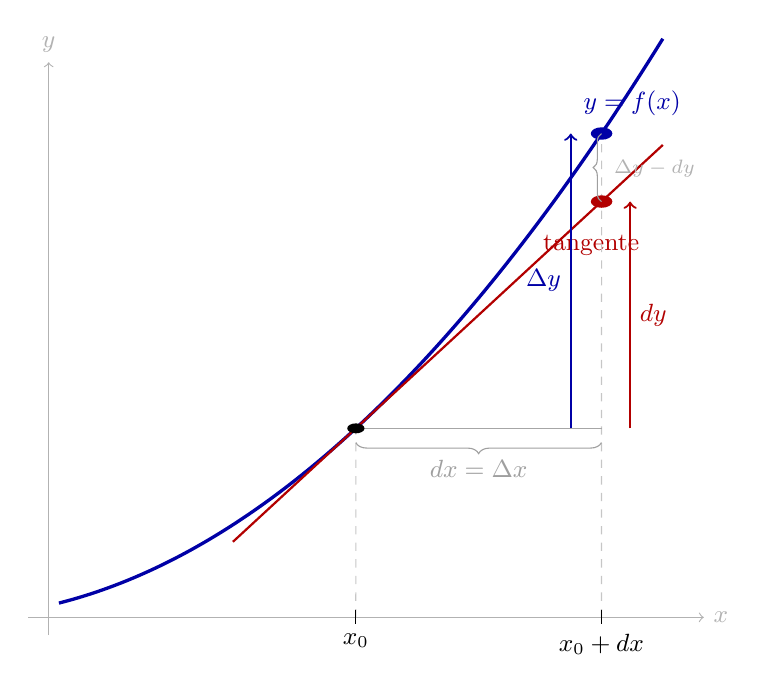
\begin{tikzpicture}[xscale=2.6, yscale=1.5, every node/.style={font=\small}]
    % Curva f(x)=0.4x^2
    \draw[blue!65!black, very thick, domain=0.55:3.5, samples=80, smooth, variable=\x]
        plot (\x, {0.4*\x*\x});
    \node[blue!65!black] at (3.35, 4.35) {$y=f(x)$};
    % Recta tangente en x0=2: y = 1.6 + 1.6(x-2)
    \draw[red!70!black, thick, domain=1.4:3.5, variable=\x]
        plot (\x, {1.6 + 1.6*(\x-2)});
    \node[red!70!black] at (3.15, 3.15) {tangente};
    % Ejes
    \draw[->, gray!60] (0.4,0) -- (3.7,0) node[right] {$x$};
    \draw[->, gray!60] (0.5,-0.15) -- (0.5,4.7) node[above] {$y$};
    % Coordenadas clave
    \coordinate (A) at (2, 1.6);      % (x0, f(x0))
    \coordinate (B) at (3.2, 4.096);  % (x0+dx, f(x0+dx)) sobre la curva
    \coordinate (T) at (3.2, 3.52);   % (x0+dx, tangente) altura 1.6+1.92
    \coordinate (H) at (3.2, 1.6);    % esquina horizontal
    % Verticales de referencia
    \draw[gray!45, dashed] (2,0) -- (A);
    \draw[gray!45, dashed] (3.2,0) -- (B);
    % Segmento horizontal dx
    \draw[gray!70] (A) -- (H);
    % Puntos
    \fill[black] (A) circle (1.2pt);
    \fill[blue!65!black] (B) circle (1.5pt);
    \fill[red!70!black] (T) circle (1.5pt);
    % Marcas en el eje x
    \draw (2,0.06) -- (2,-0.06) node[below] {$x_0$};
    \draw (3.2,0.06) -- (3.2,-0.06) node[below] {$x_0+dx$};
    % Llave para dx (bajo el segmento horizontal)
    \draw[decorate, decoration={brace, amplitude=4pt, mirror}, gray!75]
        (2,1.48) -- (3.2,1.48) node[midway, below, yshift=-3pt] {$dx=\Delta x$};
    % dy: de H a T (rise sobre la tangente)
    \draw[->, red!70!black, thick] (3.34,1.6) -- (3.34,3.52);
    \node[red!70!black, right] at (3.34, 2.56) {$dy$};
    % Delta y: de H a B (rise sobre la curva)
    \draw[->, blue!65!black, thick] (3.05,1.6) -- (3.05,4.096);
    \node[blue!65!black, left] at (3.05, 2.85) {$\Delta y$};
    % Error Delta y - dy
    \draw[decorate, decoration={brace, amplitude=3pt}, gray!75]
        (3.2,3.52) -- (3.2,4.096);
    \node[gray!60, right, xshift=1pt] at (3.2, 3.8) {\scriptsize $\Delta y - dy$};
\end{tikzpicture}
\end{center}

En la figura, $dx$ es el desplazamiento horizontal, $\Delta y$ es el ascenso real sobre la curva y $dy$ es el ascenso sobre la recta tangente. Cuanto menor sea $dx$, más pequeña es la brecha $\Delta y - dy$ entre la curva y su tangente.

La misma idea se traslada a dos variables sin más que reemplazar la recta tangente por el plano tangente. Sea $z = f(x, y)$ diferenciable. Cuando $(x, y)$ pasa de $(x_0, y_0)$ a $(x_0 + \Delta x, y_0 + \Delta y)$, el cambio real en $z$ es:
\[
\Delta z = f(x_0 + \Delta x,\, y_0 + \Delta y) - f(x_0, y_0).
\]
Igual que $\Delta y$ se aproximaba subiendo por la recta tangente, ahora $\Delta z$ se aproxima subiendo por el plano tangente. El ascenso sobre ese plano, correspondiente a los desplazamientos $dx$ y $dy$, es el diferencial total.

\begin{mydefinition}{Diferencial total}
El diferencial total de $z = f(x, y)$ en el punto $(x_0, y_0)$ es:
\[
dz = f_x(x_0, y_0)\,dx + f_y(x_0, y_0)\,dy
\]
donde $dx$ y $dy$ son variables independientes que representan los incrementos en $x$ e $y$.
\end{mydefinition}

La estructura es la misma que en una variable. Allí un solo término, $f'(x_0)\,dx$, recogía la contribución de la única dirección disponible; aquí hay una contribución por cada variable, $f_x\,dx$ en la dirección $x$ y $f_y\,dy$ en la dirección $y$, y el diferencial total es su suma. El diferencial $dz$ mide el cambio en altura sobre el plano tangente cuando $(x, y)$ se desplaza $dx$ en la dirección $x$ y $dy$ en la dirección $y$. La relación entre el cambio real y el diferencial es:
\[
\Delta z \approx dz \quad \text{cuando } dx \text{ y } dy \text{ son pequeños}
\]

En la notación general para $w = f(x_1, \dots, x_n)$, el diferencial total es:
\[
dw = \frac{\partial f}{\partial x_1}\,dx_1 + \frac{\partial f}{\partial x_2}\,dx_2 + \cdots + \frac{\partial f}{\partial x_n}\,dx_n
\]

Una aplicación directa del diferencial es la estimación de errores: si cada variable $x_i$ tiene un error de medición $dx_i$, el error propagado en $f$ se estima como $|df|$.

\textbf{Ejemplo 1.} Sea $z = x^2 y^3$. El diferencial es:
\[
dz = 2xy^3\,dx + 3x^2 y^2\,dy
\]
Si $(x, y) = (2, 1)$, $dx = 0.1$ y $dy = -0.05$:
\[
dz = 2 \cdot 2 \cdot 1 \cdot (0.1) + 3 \cdot 4 \cdot 1 \cdot (-0.05) = 0.4 - 0.6 = -0.2
\]
El cambio real es $\Delta z = (2.1)^2(0.95)^3 - 4 \approx -0.1986$, consistente con la estimación.

\textbf{Ejemplo 2.} Las dimensiones de una caja rectangular se miden con errores de hasta $0.1$ cm en cada dimensión. Si las medidas nominales son $l = 10$ cm, $w = 8$ cm y $h = 5$ cm, estimar el error en el volumen $V = lwh$.
\[
dV = wh\,dl + lh\,dw + lw\,dh = 40\,dl + 50\,dw + 80\,dh
\]
Con $|dl|, |dw|, |dh| \leq 0.1$:
\[
|dV| \leq 40(0.1) + 50(0.1) + 80(0.1) = 4 + 5 + 8 = 17 \text{ cm}^3
\]
El volumen nominal es $V = 400$ cm$^3$, con un error relativo estimado de $17/400 = 4.25\%$.

\subsection{Ejercicios}

\begin{enumerate}
    \item Halle la ecuación del plano tangente a cada superficie en el punto indicado.
\begin{enumerate}
    \item $f(x,y) = 4x^2 + y^2$ en $(1, 2)$
    \item $f(x,y) = \sqrt{x} + \sqrt{y}$ en $(4, 1)$
    \item $f(x,y) = x\sin(y)$ en $(2, \pi/6)$
\end{enumerate}

    \item Halle la ecuación del plano tangente a cada superficie en el punto indicado.
\begin{enumerate}
    \item $f(x,y) = e^{x-y}$ en $(1, 1)$
    \item $f(x,y) = \ln(x^2 + y^2 + 1)$ en $(0, 0)$
    \item $f(x,y) = \dfrac{xy}{x^2 + y^2 + 1}$ en $(1, -1)$
\end{enumerate}

    \item Determine los puntos de la superficie $z = x^2 - xy + y^2 - 2x + 4y$ donde el plano tangente es paralelo al plano $z = 2x - 4y + 1$.

    \item Halle la linealización $L(x,y)$ de cada función en el punto indicado y úsela para aproximar el valor señalado.
\begin{enumerate}
    \item $f(x,y) = \sqrt{x^2 + y^2}$ en $(3, 4)$, aproximar $f(2.97,\, 4.02)$.
    \item $f(x,y) = e^x \cos y$ en $(0, 0)$, aproximar $f(0.1,\, 0.05)$.
\end{enumerate}

    \item Use la aproximación lineal de $f(x,y) = x^y$ en $(1, 3)$ para estimar $(1.03)^{2.95}$. Compare con el valor obtenido por calculadora.

    \item Calcule el diferencial total de cada función.
\begin{enumerate}
    \item $z = x^3 \sin(2y)$
    \item $w = \dfrac{u^2 - v^2}{u^2 + v^2}$
    \item $T = e^{-r}\cos\theta$
\end{enumerate}

    \item El radio y la altura de un cilindro recto se miden como $r = 5$ cm y $h = 12$ cm, con errores de medición de hasta $0.05$ cm en $r$ y $0.1$ cm en $h$. Use diferenciales para estimar el error máximo en el cálculo del volumen $V = \pi r^2 h$.

    \item La resistencia $R$ de dos resistores en paralelo es $R = \dfrac{R_1 R_2}{R_1 + R_2}$. Si $R_1 = 80\,\Omega$ y $R_2 = 100\,\Omega$, cada uno con un error relativo de $2\%$, estime el error relativo máximo en $R$ usando diferenciales.

\end{enumerate}
